\chapter{Fourier Transforms}\label{ch:fourier}



% An excellent 
% \href{http://ocw.mit.edu/courses/physics/8-03-physics-iii-vibrations-and-waves-fall-2004/video-lectures/lecture-7/}{video}
% lecture by Walter Lewin from MIT derivation of the wave equation from first
% principles (start at 44:58 and continue to 63:50, $\sim$19~min).  We'll do
% something later in the section on seismology, but we'll be approaching it from
% stresses in a solid rather than tension in a spring.


%\begin{figure}[h]
%  \centerline{
%    
\includegraphics[width=15pc]{fourier.png}
%  }
%  \caption{Fourier. Source: Randall Munroe, \protect\url{http://www.xkcd.org}.}
%  \label{fig-cat}
%\end{figure}
\epigraph{ ``Fourier's Theorem is not only one of the most beautiful results of modern analysis, but it is said to furnish an indispensable instrument in the treatment of nearly every recondite question in modern physics.''}
{{\normalfont ---\ Lord Kelvin}}

\section*{Introduction}

While Fourier series are used to determine unknown physical fields within bounded domains, Fourier transforms serve a different purpose in geoscience: they are used to analyze, manipulate, and interpret observed data. In geophysics, we frequently work with measurements that are already known—seismograms, gravity and magnetic anomaly maps, magnetotelluric time series, or climate proxy records—but whose structure is more easily understood when expressed in terms of frequency or wavelength rather than time or space.

The Fourier transform provides a systematic way to reorder information by scale, converting a function from the time or spatial domain into the frequency or wavenumber domain. This change of representation simplifies many operations that are mathematically cumbersome in the original domain. Differentiation, integration, filtering, continuation, and convolution become algebraic operations in Fourier space, making the transform an indispensable tool for processing and interpreting geophysical data.

Fourier transforms are foundational to modern geophysical practice. They are used to identify dominant temporal or spatial scales, separate shallow from deep sources in potential field data, design and apply filters, perform upward and downward continuation, and solve certain classes of differential equations numerically. Although Fourier transforms make use of the same trigonometric functions encountered in Fourier series, their role is fundamentally different: the transform does not solve for an unknown field, but instead provides a new coordinate system in which the properties of known data are more transparent.

Because of these differences, it is important to develop a clear distinction between Fourier series and Fourier transforms. Having first examined Fourier series as a method for constructing solutions constrained by boundaries, we now turn to Fourier transforms as a general-purpose mathematical lens for geophysical data analysis.
\begin{table}[htbp]
    \centering
    \begin{threeparttable}
    \caption{The differences between Fourier series and Fourier transforms.}
    \label{tab:fs_v_ft}
    \begin{tabular}{@{}lll@{}}
        \toprule
        \textbf{Fourier Series} & \textbf{Fourier Transform} & \textbf{DFT} \& \textbf{FFT}\tnote{a}\\
        \midrule
        solves PDEs & transforms operators & approximates Fourier transforms \\
        finite domain (physics constrained) & infinite domain & finite domain (measurement-limited) \\
        boundary conditions enforced & no boundaries & boundaries implictly periodic \\
        discrete eigenvalues & continuous spectrum & discrete, resolvable frequencies \\
        \bottomrule
    \end{tabular}
    \begin{tablenotes}
        \item[a] DFT, discrete Fourier transform; FFT, fast Fourier transform.
    \end{tablenotes}
    \end{threeparttable}
\end{table}


\section{Review of Waves}

Before introducing the Fourier transform, it is useful to review the basic properties of waves and the parameters used to describe them. Waves provide a common language for many geophysical observations, including seismic motion, potential field variations, electromagnetic signals, and climate variability. Even when a signal does not appear sinusoidal, Fourier methods allow it to be represented as a combination of simple waves.

\subsection{Temporal Waves}

A simple harmonic wave that varies in time can be written as
\[
    f(t) = \mlbox[
        labelstyle={xshift=-1cm},
        linestyle={out=270,in=90, latex-}]
    {A}{amplitude}
    \cos \bigl(
    \mlbox[
        labelstyle={xshift=-1cm, yshift=-1cm, below of=m\themathLableNode},
        linestyle={out=90,in=270, latex-}]
    {\omega}{angular frequency}
    \mlbox[
        labelstyle={xshift=0.5cm},
        linestyle={out=270,in=90, latex-}]
    {t}{time}
    -
    \mlbox[
        labelstyle={xshift=1cm, yshift=-1cm, below of=m\themathLableNode},
        linestyle={out=90,in=270, latex-}]
    {\phi}{phase}
    \bigr),
\]
where the three parameters that completely describe the wave are its amplitude, frequency, and phase (Figure~\ref{fig:waveparam}$a$).
\begin{figure}[hbt]
    \centering
    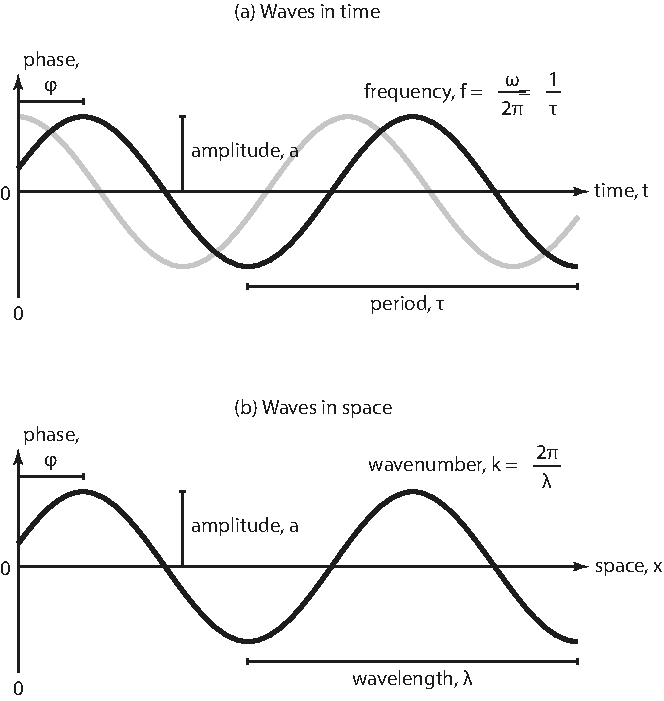
\includegraphics[]{numerical/figures/wave_parameters.pdf}
    \caption{The scale and shifting factors for waves have been given names which differ when describing temporal and spatial signals.  These waves (black) are referenced to a cosine (grey) curve.}
    \label{fig:waveparam}
\end{figure}

The angular frequency $\omega$ is related to the frequency $f$ by
\begin{equation}
    \coreeq
    \omega = 2\pi f,
\end{equation}
where frequency has units of cycles per unit time. The period $\tau$ is the time required for one complete cycle and is given by
\begin{equation}
    \coreeq
    \tau = f^{-1} = \frac{2\pi}{\omega}.
\end{equation}

In geophysics, temporal waves arise naturally in seismology, electromagnetics, and climate records, where periods often correspond to physically meaningful time scales such as wave propagation times, diffusion times, or climatic cycles.

\subsection{Spatial Waves}

An analogous expression describes a wave that varies in space,
\[
    f(t) = \mlbox[
        labelstyle={xshift=-1cm},
        linestyle={out=270,in=90, latex-}]
    {A}{amplitude}
    \cos \bigl(
    \mlbox[
        labelstyle={xshift=-1cm, yshift=-1cm, below of=m\themathLableNode},
        linestyle={out=90,in=270, latex-}]
    {k}{wavenumber}
    \mlbox[
        labelstyle={xshift=0.5cm},
        linestyle={out=270,in=90, latex-}]
    {x}{distance}
    -
    \mlbox[
        labelstyle={xshift=1cm, yshift=-1cm, below of=m\themathLableNode},
        linestyle={out=90,in=270, latex-}]
    {\phi}{phase}
    \bigr),
\]
where the wavenumber $k$ controls the spatial scale of the variation (Figure~\ref{fig:waveparam}). The wavelength $\lambda$ is the distance over which the wave completes a full cycle and is related to wavenumber by
\begin{equation}
    \coreeq
    k = \frac{2\pi}{\lambda}.
\end{equation}

Spatial waves are particularly important in gravity, magnetic, thermal and electromagnetic studies, where wavelength is closely linked to source depth or feature width: long wavelengths are typically associated with deeper sources, while short wavelengths reflect shallow structure.

\subsection{Amplitude, Frequency, and Phase}

Both temporal and spatial waves are fully described by three quantities:
\begin{description}
    \item[Amplitude], which controls the strength of the signal;
    \item[Frequency or wavenumber], which controls the scale of variation;
    \item[Phase], which controls the location of features in time or space.
\end{description}

In temporal problems, frequency is commonly expressed in hertz (cycles per unit time), while in spatial problems the analogous quantity is the wavenumber, which describes cycles per unit distance. The inverse of frequency or wavenumber defines the period or wavelength, quantities that are often more intuitive in a geological context because they correspond directly to time scales or spatial scales of structure.

The phase parameter determines where peaks, troughs, or zero crossings occur. Two waves may have identical amplitude and frequency but differ entirely in appearance due to differences in phase. In geophysics, phase often carries geometric information, such as the location of a source or the alignment of a signal relative to a reference point.

A key observation is that an individual wave, regardless of how finely it is sampled, can be represented exactly using only these three parameters. A time or spatial series containing thousands of sampled values can therefore be compressed into just three numbers if it consists of a single wave. This idea underlies the utility of Fourier methods. Hence, wave descriptions, and Fourier Tranforms, provide a highly compact representation of information.

Most geophysical signals are not composed of a single wave, but rather a superposition of many waves with different frequencies or wavenumbers and phases. The Fourier transform determines these parameters for all constituent waves simultaneously, producing spectra that describe how amplitude and phase vary with scale. For signals dominated by a limited range of scales, this representation can dramatically reduce the complexity of the problem while preserving the essential physical information. Fourier transforms aid identifying dominant frequencies or wavelengths, assessing where noise becomes important, and applying scale-dependent operations (filters) in a controlled and physically interpretable way.


% \section{Introduction}

% In many applications of geophysics we deal with problems where we may know what a function looks like, but not have a mathematical expression to deal with it.
% Examples include
% \begin{enumerate}
%     \item a seismogram, the ground motion (displacement as a function of time) associated with an earthquake;

%     \item a map of the gravity field (or magnetic field, or heat flow, etc.);

%     \item variations in the electric and magnetic field observed at the surface of Earth (magnetotellurics); and

%     \item air temperature changes at the surface of Earth.
% \end{enumerate}
% The first three of the examples relate to temporal variations and one to spatial variations of complex functions that may not be possible to write down as a simple mathematical function.  These problems are not limited to geophysics as they find many applications in other geologic fields as well (particularly, paleoclimate and paleoenvironmental studies).  For example, isotope records in sediment or ice cores can be looked at as a discrete function of that record in time.

% We need to be able to analyze these sorts of data.  Paleoclimate data may be the easiest to consider as an example.  Some major climatic drivers are cyclic including solar energy input (think day/night, yearly variations, and 22 year sunspot cycle), orbital (Milankovitch) cycles (precession, obliquity, and eccentricity of orbit).  For gravity as well as climate, lunar and solar tides are also cyclic.  So for many systems, we may wish to try and find cyclical variations that may otherwise be obscured by additional geological/geophysical processes.

% For spatial variations in potential fields, we are often interested in finding the depth to sources/targets or are interested in isolating near surface versus deep causes.  A problem that also arises with potential fields includes leveling airborne data (gravity, magnetics, radiometrics) flown at different altitudes.

% The analysis required for each of these processes (and many more) require expressing our data as a function.  However, since there is no simple mathematical way to describe our data so we need to develop one.  Fortunately, methods to describe an arbitrary function as a set of simple functions has already been devised.  The most common method utilizes a set of sine and/or cosine functions.  We call this method of constructing arbitrary functions in this way Fourier series.  An extension of the Fourier series is the Fourier transform, which allows us to remove time (or spatial) variables in favor of frequency (or wavenumber) variables, which can make the math far simpler.

% \section{Waves}

% It is possible to write a function as a combination of two or more functions, e.g., $f(x) = g(x) + h(x)$.  What we want to do is write an arbitrary function as a combination of a set of well defined functions.  Ideally, they will share some similar characteristics that will make certain mathematical operations simpler.  A minimal set of parameters is also advantageous, we want our functions to be relatively simple.  Smooth functions are desirable (we can even produce discontinuous functions so long as we use an infinite number of functions).  It is also preferred if our functions are orthogonal and form a basis (see box below).

% The trigonometric functions sine and cosine are ideal candidate functions to build other functions.  First, each function looks relatively similar in form.  Second, one only needs a minimal set of parameters to describe them (amplitude and frequency).  And as will soon see, they form an orthogonal basis.

% Fourier series and Fourier transforms rely on the periodic properties of trigonometric functions and the ease with which they can be scaled and stretched.  A description of the wave parameters are described in 

% We can use these sine and cosine waves to build any function we desire.  An example of a slightly more complex function can be seen in Figure~\ref{fig:cossum}.  The constructed function is a set of 32 cosine functions,
% \begin{equation*}
%     f(x) = \sum_k = 1^32 \cos (k x) .
% \end{equation*}
% While some of the periodicity of the cosines is still evident, it is clear that the function is becoming more and more peaked as terms are added and the amplitude of the ``side lobes'' (the little squiggles about the main peak)
% become smaller.
% \begin{figure}[hbt]
%     \centering
%     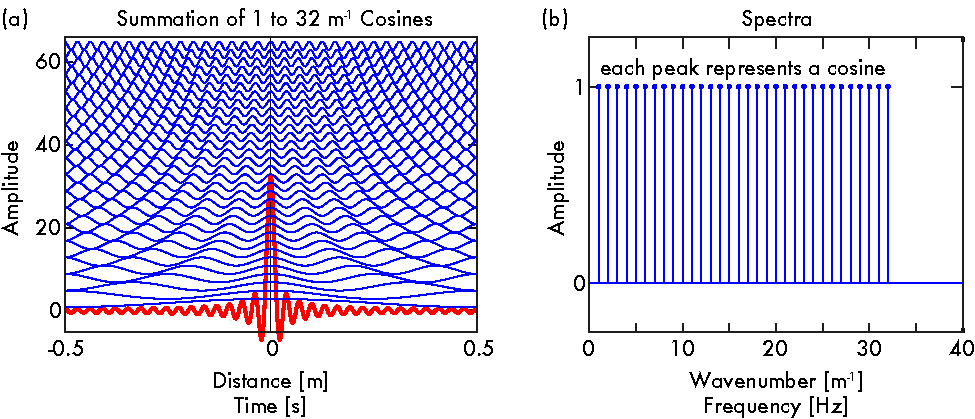
\includegraphics[]{numerical/figures/cosine_sum.pdf}
%     \caption{Demonstrating the construction of a new function using 32 cosine functions. (a) The individual functions in blue are used to construct the function in red. (b) The amplitude spectrum associated with the cosines in (a) showing the frequencies/wavenumbers and their amplitudes (all have the same amplitude).}
%     \label{fig:cossum}
% \end{figure}

\section{Continuous Fourier Transform}

The {\bf continuous Fourier transform} (FT) was first published by Joseph Fourier in 1822 and is used to decompose a function into periodic functions.  FT's find a wide array of uses from identifying the composition of stars (spectroscopy) to cell phone transmissions to image processing to solving differential equations.

Sometimes shorthand notation for a FT is given by 
\[
    h(\xi) \overset{\mcal{F}}{\longleftrightarrow} H(\nu),
\]
where $h(\xi)$ is a function with the FT $H(\nu)$.  Generally, $\xi$ is either time or a spatial coordinate(s) and $\nu$ is the frequency or wavenumber(s) (spatial analog to frequency).  {\bf The forward transform} goes from left to right and {\bf inverse transform} from right to left.

Forward transform
\begin{equation}
    \workeq
    \mcal{F} [h(\xi)] = H(\nu) = 
    \int_{-\infty}^{\infty} h(\xi)
    \exp [ -i 2 \pi (\nu \cdot \xi) ]\, d\xi,
\end{equation}
Inverse transform
\begin{equation}
    \workeq
    \mcal{F}^{-1} [H(\nu)] = h(\xi) = 
    \int_{-\infty}^{\infty} H(\nu)
    \exp [ i 2 \pi (\nu \cdot \xi) ]\, d\nu.
\end{equation}

The complex number $i = \sqrt{-1}$ (Figure!\ref{fig-eipi}).  Note that $j$ is occasionally used as the complex number, particularly in electrical engineering texts.  Recall that $\exp( i \theta ) = \cos(\theta) + i \sin(\theta)$, hence, a FT and its inverse can be represented by a series of trigonometric functions with varying amplitudes and frequencies.
\begin{eqnarray*}
    \exp( i 2 \pi f t ) & = &\cos(2 \pi f t) + i \sin(2 \pi f t) \mbox{ and} \\
    \exp( - i 2 \pi f t ) & = &\cos(2 \pi f t) - i \sin(2 \pi f t).
\end{eqnarray*}

FT's can be performed on temporal (i.e.  {\bf time-domain}) or spatial (i.e.  {\bf spatial-domain}) processes converting a function into the {\bf frequency-domain}.

For example, in two spatial dimensions the Fourier transform is written as
\[
    H(k_x,k_y) = \int_{-\infty}^{\infty}\int_{-\infty}^{\infty}
    h(x,y) \exp [ -i 2 \pi (k_{x}x + k_{y} y) ]\,
    dx\, dy,
\]

\subsection{Interpretation of Variables}

The mathematical form of the Fourier transform does not depend on the physical meaning of the independent variable. The same transform applies whether $\xi$ represents time, space, or another coordinate.

When $\xi = t$, the Fourier transform converts a time-domain signal into a frequency-domain representation, where frequency describes the rate of temporal variation. The inverse of frequency corresponds to a characteristic timescale or period.

When $\xi = x$ (or more generally $\vb{x}$), the Fourier transform converts a spatial signal into a wavenumber-domain representation, where wavenumber describes the rate of spatial variation. The inverse of wavenumber corresponds to wavelength, a directly interpretable measure of spatial scale.

From a geophysical perspective, this distinction is interpretive rather than mathematical. Short periods or wavelengths describe rapid or fine-scale variations, while long periods or wavelengths describe slow or broad-scale structure. In many applications, wavelength is closely related to depth sensitivity, while frequency is linked to timescales of physical processes.

Because the underlying mathematics is identical, Fourier methods provide a unified language for analyzing both temporal and spatial data.

\section{Amplitude and Phase}

A Fourier transform expresses a function as a sum of complex exponentials, each characterized by an amplitude and a phase at a particular frequency or wavenumber. These two quantities describe fundamentally different aspects of a geophysical signal, and it is essential to understand their physical meaning before applying Fourier-domain operations.

A forward Fourier transformed function is complex and therefore can be written as,
\begin{equation}
    H(\nu) = A(\nu) + iB(\nu) = \abs{H(\nu)} \exp [ i \phi(\nu) ],
\end{equation}
where $A(\nu)$ and $B(\nu)$ are the real and imaginary parts of $H(\nu)$, respectively.  We often refer to the {\bf amplitude spectrum}, $\abs{H(\nu)}$, and the {\bf phase spectrum}, $\phi(\nu)$  of a signal.  We can write these two spectra in terms of the real and imaginary parts of $H(\nu)$,
\begin{eqnarray}
    \workeq
    \abs{H(\nu)} & = & [A^{2}(\nu) + B^{2}(\nu)]^{1/2}, \mbox{ and}\\
    \phi(\nu) & = & \tan^{-1}\left[\frac{B(\nu)}{A(\nu)} \right].
\end{eqnarray}is on derivation—focus on interpretation)

In geophysics, Fourier transforms are most often applied to signals or fields that are already known through observation, such as seismograms, gravity and magnetic anomaly maps, or electromagnetic time series. The Fourier domain does not introduce new information; rather, it reorganizes existing information in a way that makes scale-dependent behavior explicit.

In this representation, the \textbf{amplitude} describes how much of a particular frequency or wavelength is present in the signal, while the \textbf{phase} describes where that component is located in time or space. Both are required for a complete description of the original signal.

\subsection{What Amplitude Tells Us}

The amplitude spectrum measures the strength of oscillations at different frequencies or wavenumbers. In spatial problems, it indicates how much variability exists at different length scales; in temporal problems, it shows how energy or variance is distributed across time scales.

Amplitude is often closely tied to physical processes. For example, in potential field data, large amplitudes at long wavelengths are commonly associated with deep or laterally extensive sources, while strong short-wavelength amplitudes suggest shallow structure. In seismic or electromagnetic time series, amplitude spectra can be used to identify dominant frequencies, attenuation effects, or the frequency range over which noise begins to dominate the signal.

Because amplitude reflects the relative importance of different scales, amplitude spectra are widely used for filtering, smoothing, and scale separation.

\subsection{What Phase Tells Us}

Whereas amplitude describes \emph{how much} of each component is present, phase describes \emph{where} it occurs. Phase controls the alignment of peaks, troughs, and zero crossings in time or space and therefore carries information about geometry, location, and waveform shape.

Two signals can have identical amplitude spectra but look entirely different in the time or spatial domain if their phase spectra differ. In geophysical applications, phase often encodes critical information such as the position of sources, the timing of arrivals, or the sharpness of boundaries.

Phase behavior is particularly important in applications such as migration, deconvolution, and reduction-to-the-pole transformations, where the goal is often to relocate or re-center physical features rather than simply emphasize or suppress particular scales.

\subsection{Why Both Amplitude and Phase Matter}

Amplitude and phase together provide a complete description of a Fourier-transformed signal. Amplitude alone describes the distribution of energy or variance across scales, but without phase information it cannot reconstruct the original signal. Phase, in turn, determines the geometric arrangement of those components but does not indicate their relative strength.

This distinction has important practical consequences. Operations that modify only the amplitude spectrum tend to change the smoothness or scale content of a signal while preserving its geometry. Operations that modify phase, by contrast, can shift, distort, or relocate features in time or space, often with significant implications for interpretation.

Understanding the distinct roles of amplitude and phase is therefore crucial for interpreting Fourier-domain results and for anticipating the effects of filtering, continuation, and other spectral operations introduced later in this chapter.


\section{Discrete and Fast Fourier Transforms}

\subsection{Discrete Fourier Transform (DFT)}

Geophysical data are almost always discrete. Measurements are made at specific locations in space or at specific times, with a finite sampling interval and a finite record length. Seismograms are sampled at fixed time steps, gravity and magnetic data are collected at discrete stations or along flight lines, and electromagnetic measurements are recorded at discrete times. As a result, the continuous Fourier transform must be replaced by a discrete formulation when working with real data.

The discrete Fourier transform (DFT) was first developed, although never published, by Heinrich Gauss in 1805 to describe the orbits of asteroids using discrete observations. It was later rediscovered by Cooley and Tukey in 1965 in a form suitable for efficient computation. In most scientific applications, including geophysics, the DFT is far more practical than the continuous Fourier transform because it operates directly on discretely sampled, finite-length data.

\subsubsection*{Finite Sampling and Record Length}

The DFT addresses two fundamental constraints of observed data:
\begin{itemize}
    \item the data are sampled at discrete intervals, and
    \item the data record has finite length.
\end{itemize}

Rather than requiring integration over an infinite domain, the DFT replaces integrals with finite sums and continuous functions with sequences of sampled values.

For a discrete dataset
\[
    \vb{d} = \{d_0, d_1, \ldots, d_{N-1}\},
\]
the DFT produces an equally sized set of complex coefficients,
\[
    \vb{D} = \{D_0, D_1, \ldots, D_{N-1}\},
\]
which describe the contribution of discrete frequencies or wavenumbers to the signal.

\subsubsection*{Definition of the DFT}

The forward discrete Fourier transform is defined as
\begin{equation}
    \workeq
    D_k = \sum_{n=0}^{N-1} d_n 
    \exp \left[-\frac{i 2 \pi}{N} k n\right],
    \quad k = 0, \ldots, N-1,
    \label{eq-dft}
\end{equation}
and the inverse transform as
\begin{equation}
    \workeq
    d_n = \frac{1}{N}\sum_{k=0}^{N-1} D_k 
    \exp \left[\frac{i 2 \pi}{N} k n\right],
    \quad n = 0, \ldots, N-1.
    \label{eq-idft}
\end{equation}

Together, these equations provide a one-to-one mapping between the data sequence and its discrete frequency-domain representation.

Note that within \textsc{Matlab} and many other programming languages, array indices start at 1 rather than 0. In such cases, the sums are written from $1$ to $N$, with the substitutions $n \rightarrow n-1$ and $k \rightarrow k-1$.

\subsubsection*{Discrete Frequencies}

Equations \ref{eq-dft} and \ref{eq-idft} implicitly assume unit sample spacing. To relate the discrete index $k$ to a physical frequency or wavenumber, the sampling interval $\Delta \xi$ must be introduced.

For a record of length $N\Delta \xi$, the discrete frequencies are given by
\begin{equation}
    \workeq
    \nu_k = \frac{k}{N\,\Delta \xi},
    \quad k = 0, \ldots, N-1.
\end{equation}

The sampling rate controls the highest frequency that can be unambiguously represented, which we call the \textbf{Nyquist frequency},
\begin{equation}
    \coreeq
    \nu_{\mathrm{Ny}} = \frac{1}{2\,\Delta \xi}.
\end{equation}
Frequency components higher than the Nyquist frequency cannot be represented correctly and instead are folded back into lower frequencies. This folding is the origin of aliasing and is an unavoidable consequence of undersampling (Section~\ref{sec:aliasing}).

\subsubsection*{Implicit Periodicity}

An important assumption of the DFT is that the discrete data record is treated as one period of a periodic function. In other words, the data sequence is assumed to repeat indefinitely outside the observed interval.

This implicit periodicity can lead to artificial discontinuities at the boundaries of the record, particularly if the first and last samples do not match smoothly. The consequences of this assumption, including spectral leakage and the need for windowing, will be discussed later in the chapter.

\subsubsection*{FFT as a Computational Algorithm}

The fast Fourier transform (FFT) is not a different transform, but an efficient algorithm for computing the DFT. While the direct evaluation of the DFT requires $\mathcal{O}(N^2)$ operations, FFT algorithms reduce the computational cost to $\mathcal{O}(N \log N)$.

Because of this dramatic improvement in efficiency, FFTs make Fourier analysis practical for large geophysical datasets and are the standard method used in modern data processing. Conceptually, however, the FFT produces exactly the same result as the DFT defined in Equations~\ref{eq-dft} and~\ref{eq-idft}.

\subsection{Positive and Negative Frequencies}

Fourier transforms of real-valued data contain both positive and negative frequencies. This feature often causes confusion, but it arises naturally from the mathematical form of the transform rather than from any additional physical signal.

Fourier representation is based on complex exponentials of the form $e^{\pm i2\pi\nu\xi}$. A real sinusoidal function requires both the positive- and negative-frequency exponentials to be represented exactly. As a result, negative frequencies are not independent physical components but are the mathematical counterparts required to construct real-valued signals.

For any real-valued function $f(\xi)$, the Fourier transform satisfies Hermitian symmetry,
\[
F(-\nu) = F^*(\nu),
\]
where $^*$ denotes complex conjugation. Consequently, the amplitude spectrum is symmetric about zero frequency, while the phase spectrum is antisymmetric. All independent spectral information is therefore contained in the positive frequencies.

In geophysical applications, it is common to interpret only the non‑negative frequencies or wavelengths, since negative frequencies do not correspond to additional physical scales. Their presence ensures that inverse transforms return real-valued fields.

Negative frequencies become explicitly important when working with complex-valued signals or phase-sensitive operations, such as analytic signal construction, polarization analysis, or directional wavefield decomposition. Otherwise, they serve primarily as a mathematical requirement of the Fourier representation.

\section{Sampling and Aliasing}\label{sec:aliasing}

\subsection{Consequences of Undersampling}

Geophysical signals are often continuous in time or space, but they must be recorded digitally as a sequence of discrete samples. The sampling interval therefore plays a fundamental role in determining what information can be represented faithfully.

When a signal is undersampled, high-frequency content is misrepresented as lower-frequency content. This distortion is often not obvious and can be difficult to detect because the aliased signal appears internally consistent.

The term \emph{aliasing} comes from the Latin word \emph{alias}, meaning ``otherwise'' or ``at another time,'' and in modern usage often refers to a false or assumed name. In much the same way, aliased frequencies--frequencies \emph{higher} than the Nyquist frequency---masquerade as lower-frequency (longer wavelength) components that were not present in the original signal.

The effects of aliasing are severe and irreversible. Four key consequences are worth emphasizing:
\begin{enumerate}
  \item \textit{``You can't always get what you want.''} Frequency components above the Nyquist frequency are not contained correctly in the sampled data.
  \item \textit{``You get something else instead.''} High-frequency energy appears artificially at lower frequencies, creating spurious signals.
  \item \textit{``You don't know you've made a mistake.''} Aliased data often appear smooth and reasonable, masking the error.
  \item \textit{``It's too late to fix it.''} Once data have been sampled inadequately, the lost information cannot be recovered.
\end{enumerate}

These properties make aliasing particularly dangerous in geophysics, where interpretations often rely on subtle variations in amplitude, frequency content, or spatial scale.  Inadequate sampling leads to aliasing, a serious and often subtle source of error in geophysical analysis.

\subsection{Aliasing Example}

A familiar everyday example is the apparent backward rotation of wheels on a rapidly moving vehicle. As the rotation rate increases, the wheels may appear to slow, stop, or reverse direction. This visual illusion arises because the image is sampled by the human visual system at discrete time intervals, resulting in aliasing. Similar effects can be observed in rotating fan blades or helicopter rotors.

An illustration of aliasing in a sampled time series is shown in Figure~\ref{fig:aliasing}. As the sampling interval becomes too large, the reconstructed signal no longer reflects the true frequency content of the original waveform.

\begin{figure}[hbt]
    \centering
    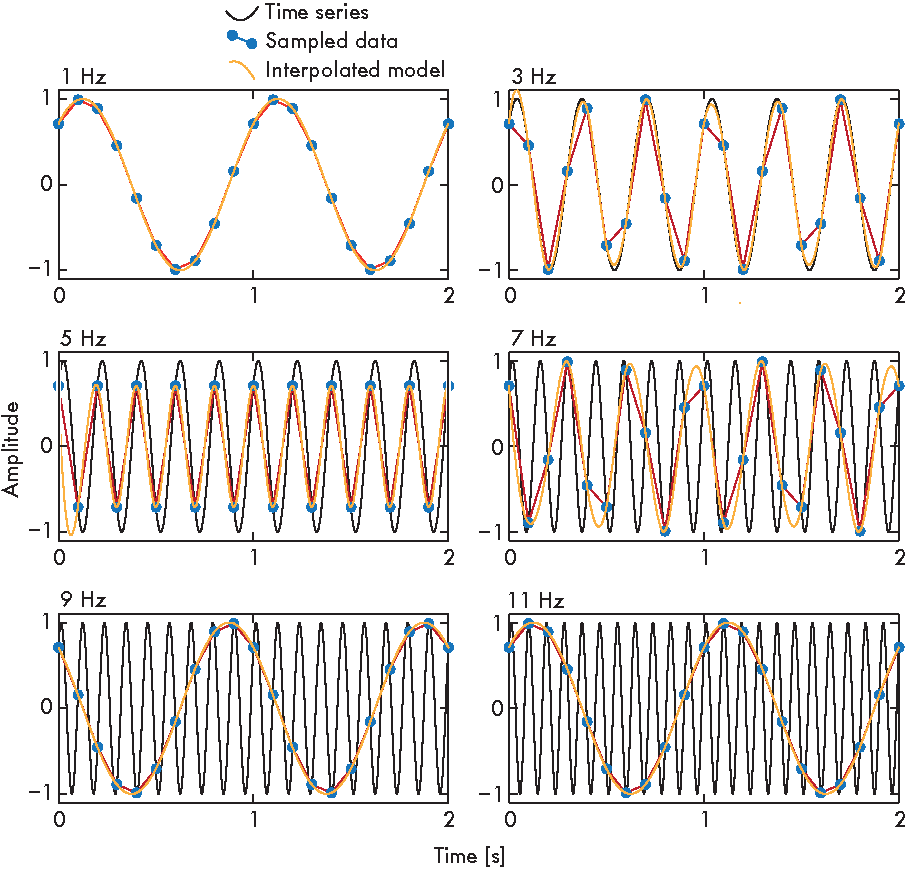
\includegraphics[]{numerical/figures/aliasing.pdf}
    \caption{Demonstration of aliasing. As the frequency of the time series increases and exceeds the Nyquist frequency (5~Hz), the interpolated signal no longer reproduces the original frequency but instead appears as a lower-frequency wave.}
    \label{fig:aliasing}
\end{figure}

\subsection{Nyquist is not enough}

The Nyquist frequency represents a \emph{theoretical} limit, not a guarantee of reliable recovery.  Its derivation assumes exactly periodic sampling, adequate phase coverage, and signal amplitudes that are large compared to noise. In practice, these assumptions are rarely met. Sampling near the nodal points of a waveform can make even sub-Nyquist signals difficult to identify, and phase rapidly becomes under-constrained as one approaches the Nyquist frequency, $\nu_{\mathrm{Ny}}$ (Figure~\ref{fig:nyquist}).

Nyquist therefore defines the maximum frequency that is theoretically representable, not the maximum frequency that can be robustly recovered from data. Near $\nu_{\mathrm{Ny}}$, each cycle is sampled by very few points, such that any pair of samples is nearly equally likely to fall anywhere on the waveform. As a result, small sampling or timing errors can produce large phase errors and a systematic underestimation of amplitude (Figure~\ref{fig:nyquist}b). While amplitude may still be detectable close to the Nyquist frequency, phase information rapidly degrades and becomes effectively meaningless (Figure~\ref{fig:nyquist}c).

In the worst case, sampling occurs exactly at the nodal points of the wave, yielding zero measured amplitude and an apparent phase offset of $180^\circ$ relative to the true signal.  This behaviour is particularly important for traveltime analysis, phase-sensitive inversions, and spectral interpretations in noisy data.

For practical purposes, a more conservative upper limit on usable frequency is often required.  A common rule of thumb is that reliable phase and amplitude recovery typically require at least four samples per cycle (Figure~\ref{fig:nyquist}b, blue line), corresponding to a frequency of approximately
\[
    \nu_{\mathrm{practical}} \approx \frac{1}{4\Delta\xi}.
\]
At this sampling density, a waveform is sufficiently over-resolved that phase estimates are stable against noise, timing errors, and unfavourable sample placement relative to nodal points.  Frequencies between $1/(4\Delta\xi)$ and the Nyquist frequency may be representable in principle, but their interpretation should be treated with caution.
\begin{figure}[htbp]
    \centering
    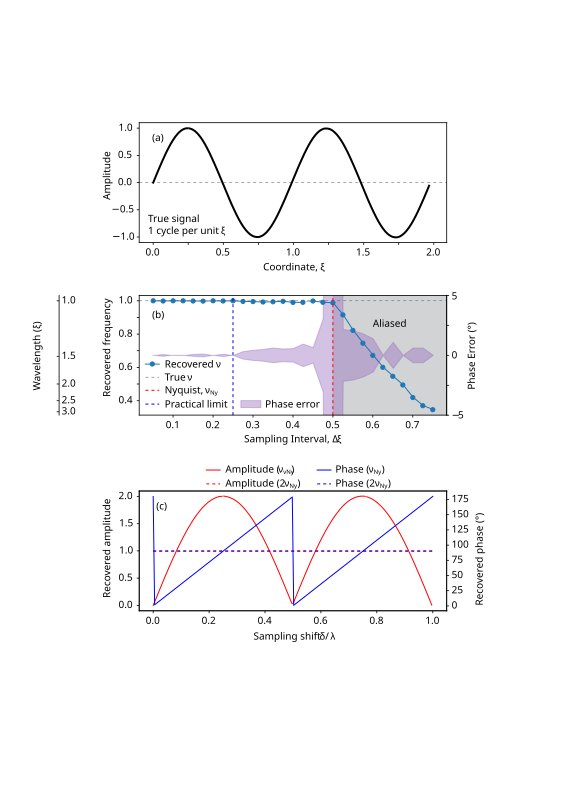
\includegraphics{numerical/figures/nyquist.eps}
    \caption{An exploration of sampling and Fourier transform results around the Nyquist frequency, $\nu_{Ny}$. (a) The true wave, a sinusoid with one cycle per unit coordinate length. Over- and under-sampled waves are shown in blue and red respectively. (b) Recovered frequency relative to sampling frequency.  Sampling intervals larger than the Nyquist alias the signal resulting in incorrect frequency estimates.  Hence under sampled wave in (a) is aliased. Also shown on (b) is the phase error envelope represents the maximum and minimum error possible for a given sampling interval.  The amplitude error is similarly shaped with an amplitude error generally less than 2\%. (c) Sampling at the Nyquist frequency with a shift, $\delta$, of the first sampling point relative to the wavelength, $\lambda$. At the $\nu_{Ny}$, the sinusoidal basis becomes degenerate; amplitude estimates are biased because all energy collapses into a single basis function causing a large error.  Phase estimates are also poor at $\nu_{Ny}$ with potential errors of $\pm90^\circ$.}  
    \label{fig:nyquist}
\end{figure}

\subsection{Preventing Aliasing}

Because aliasing cannot be corrected after sampling, it must be addressed during data acquisition. Two approaches are commonly used:
\begin{enumerate}
  \item \textbf{Survey design.} Anticipate the range of frequencies or wavelengths expected in the signal and choose a sampling interval small enough to exceed the Nyquist requirement.
  \item \textbf{Prefiltering.} If sufficiently high sampling rates are impractical, analog or digital low-pass filters can be applied before digitization to remove frequency components above the Nyquist frequency.
\end{enumerate}

Careful attention to sampling is essential in the design of geophysical surveys and monitoring systems. Many common processing problems, including spurious trends and misleading spectral features, can often be traced back to inadequate sampling at the acquisition stage.


\section{Convolution}

Convolution is a central concept in signal processing and underlies many common operations in geophysics, including filtering, smoothing, instrument response correction, and wavelet modeling. Understanding convolution is essential before introducing Fourier-domain filtering and deconvolution.

\subsection{Definition of Convolution}

Convolution is a mathematical operation that describes how one function modifies another. Given two functions $f(\xi)$ and $g(\xi)$, their convolution is defined as
\begin{equation}
    \coreeq
    (f * g)(\xi) = \int_{-\infty}^{\infty} f(\eta)\, g(\xi - \eta)\, d\eta .
\end{equation}

The value of the convolution at position $\xi$ is obtained by reversing one function, shifting it by $\xi$, multiplying it pointwise with the other function, and integrating the product over the entire domain. The result is a new function that combines the properties of both $f$ and $g$.

\subsection{Physical Meaning of Convolution}

Convolution appears whenever the value of a quantity at a given location or time depends on a weighted combination of nearby values. In geophysics, this situation arises frequently.

Conceptually, $f(\xi)$ represents an input or ideal signal, $g(\xi)$ represents a response function or kernel, and the convolution $f * g$ represents the observed or modified signal. The kernel $g$ determines how information from neighboring points contributes to the value at $\xi$. If $g$ is sharply peaked, the convolution closely resembles the original function. If $g$ is broad, the resulting signal is smoothed over a wider region.

An intuitive interpretation of convolution is as a weighted average. If the kernel $g(\xi)$ is non-negative and normalized such that
\[
    \int_{-\infty}^{\infty} g(\xi)\, d\xi = 1,
\]
then the convolution computes a local average of $f$, weighted according to the shape of $g$.

Different kernels produce different averaging behavior. A Gaussian kernel results in smooth, localized averaging; a boxcar kernel produces a simple running mean; and long-tailed kernels mix information over larger distances or longer times. This interpretation is directly relevant to smoothing, diffusion, and upward continuation in geophysics.

Convolution can also be interpreted as the response of a system to an input. If a system has a characteristic response $g(\xi)$, then convolving that response with an input signal produces the system's output. 

In geophysics, convolution naturally appears in many contexts, including seismic source wavelets modifying reflectivity, instrument responses shaping recorded data, spatial averaging introduced by finite sensor footprints, and diffusion processes spreading localized anomalies. A seismogram (Chapter~\ref{ch:seismology}) is a convolution between the source, its path through Earth, the attenuation and the receiver response function. In each case, convolution describes how structure is transferred across scales. 

\subsection{Convolution in the Fourier Domain}

Direct evaluation of the convolution integral is computationally expensive. For discretely sampled data with $N$ points, a numerical convolution requires $\mathcal{O}(N^2)$ operations, since each output sample depends on contributions from many input samples. This computational burden motivates the use of Fourier transforms, which provide a far more efficient way to evaluate convolutions, $\mathcal{O}(N \log N)$.

A key result of Fourier analysis is the convolution theorem, which states that convolution in the original domain corresponds to multiplication in the Fourier domain. Let
\[
    F(\nu) = \mathcal{F}\{f(\xi)\}, \qquad
    G(\nu) = \mathcal{F}\{g(\xi)\}.
\]
Then,
\[
    \mathcal{F}\{f * g\} = F(\nu)\,G(\nu),
\]
or equivalently,
\[
    f * g = \mathcal{F}^{-1}\!\left\{F(\nu)\,G(\nu)\right\}.
\]

This result is profound: a complicated integral operation in space or time becomes a simple pointwise multiplication in the Fourier domain.

Fourier-domain filtering is simply convolution expressed efficiently. When a filter $H(\nu)$ is applied in the Fourier domain,
\[
    \tilde{F}(\nu) = H(\nu)\,F(\nu),
\]
the corresponding operation in the original domain is convolution,
\[
    \tilde{f}(\xi) = f(\xi) * h(\xi),
\]
where $h(\xi) = \mathcal{F}^{-1}\{H(\nu)\}$ is the filter kernel.

Thus, the shape of the filter in frequency or wavenumber space determines the shape of the convolution kernel in time or space. This dual interpretation is critical for understanding the consequences of filtering.

A central lesson is that sharp spectral filters produce broad, oscillatory kernels, while smooth spectral filters produce compact, localized kernels. For example, an ideal low-pass filter with an abrupt cutoff yields a kernel that oscillates indefinitely in the original domain, whereas a Gaussian low-pass filter produces a smoothly decaying kernel.

This relationship explains why abrupt spectral truncation leads to ringing and overshoot near discontinuities. Such effects are not numerical artifacts, but a direct and predictable consequence of convolution with a long-range oscillatory kernel.

Fourier transforms do not alter the physical meaning of convolution; they simplify its execution and interpretation. By working in the Fourier domain, convolution becomes multiplication, scale dependence becomes explicit, filtering operations become computationally efficient, and issues of stability and noise amplification can be assessed algebraically.

For these reasons, Fourier transforms are indispensable tools for understanding and applying convolution-based operations throughout geophysics.


\section{Filtering}

Fourier transforms allow many common operations on geophysical data to be performed efficiently by modifying the amplitude and/or phase spectra. Working in the Fourier domain often simplifies these operations, turning convolution, differentiation, and filtering into algebraic manipulations. However, not all Fourier-domain operations affect data in the same way.

It is essential to distinguish between \textbf{amplitude filters}, which modify the relative importance of different scales, and \textbf{phase filters}, which alter the spatial or temporal alignment of features. These two classes of operations have very different physical consequences and must be interpreted with care.

\subsection{Amplitude Filters (Scale-Selective Operations)}

Amplitude filters modify how much of each frequency or wavelength contributes to the signal, while leaving the phase unchanged. Because phase controls geometry, amplitude-only filtering preserves the spatial or temporal arrangement of features but changes the smoothness or resolution of the data.
\[
    H(\nu) = A(\nu),
\]

Amplitude filters operate by altering the magnitude spectrum of a Fourier-transformed signal. Long-wavelength components can be emphasized or suppressed independently of short-wavelength components, making these filters relatively straightforward to interpret physically.

An ideal low-pass filter can be defined as
\[
    H(\nu) =
    \begin{cases}
        1, & |\nu| \le \nu_c, \\
        0, & |\nu| > \nu_c,
    \end{cases}
\]
but such filters are rarely used in practice.

The discontinuity in $H(\nu)$ introduces oscillatory behavior in the filtered signal near sharp transitions. These oscillations are a manifestation of the Gibbs phenomenon, which arises whenever sharp spectral cutoffs are applied to signals with discontinuities or strong gradients.

Common amplitude filters include low-pass filters, which emphasize long wavelengths and suppress short wavelengths; high-pass filters, which do the opposite; and band-pass or band-stop filters, which isolate or remove specific ranges of scale. Spectral smoothing and tapering in frequency or wavenumber space are also amplitude-filtering operations.  Figure~\ref{fig:filtering} illustrates the basic idea. 
\begin{figure}[hbt]
    \centering
    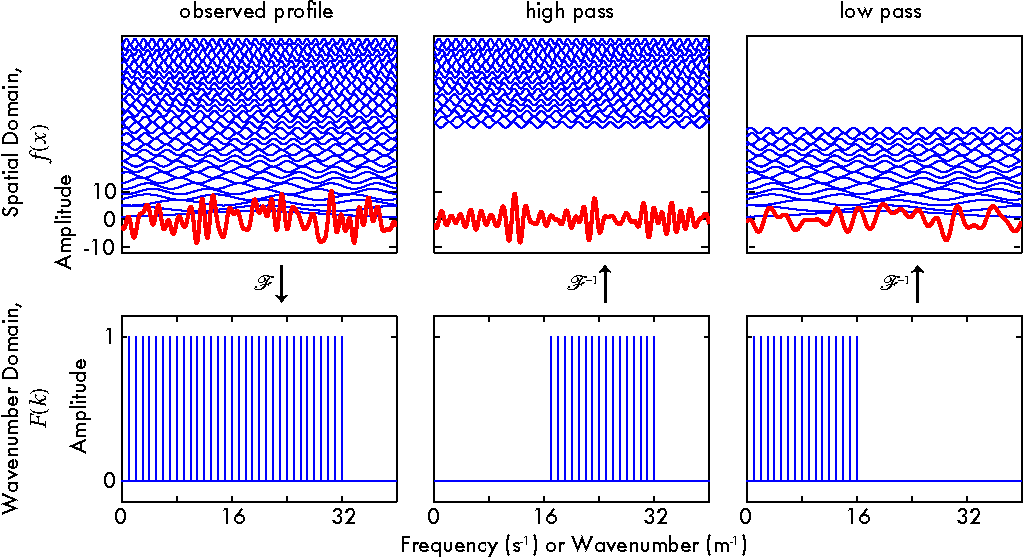
\includegraphics[]{numerical/figures/filtering.pdf}
    \caption{Use of Fourier transforms to filter a time series. The original signal can be separated by frequency or wavenumber to examine short- and long-period components individually.}
    \label{fig:filtering}
\end{figure}

In geophysical applications, amplitude filters are often used to separate regional and residual gravity fields, distinguish shallow from deep magnetic sources, reduce noise in seismic or magnetotelluric data, or emphasize characteristic length scales associated with geological structure.

Despite their apparent simplicity, amplitude filters must be applied cautiously. Filtering irreversibly removes information, and overly aggressive filtering may eliminate physically meaningful signals. The shape of the filter response is also important: sharp cutoffs can introduce artifacts, while smoother roll-offs generally produce more stable results.
\[
    A(\nu) = \exp\!\left(-\frac{\nu^2}{\nu_c^2}\right)
\]

\[
    A(\nu) =
    \exp\!\left[-\frac{(\nu-\nu_0)^2}{\sigma^2}\right]
\]
\[
    \arg\bigl(\tilde{F}(\nu)\bigr)=\arg\bigl(F(\nu)\bigr),
\]

\subsection{Phase and Mixed Filters (Geometry-Altering Operations)}

Phase filters modify where features appear in time or space and therefore directly affect geological interpretation. Unlike amplitude filters, phase-altering operations do not merely change the relative contribution of scales, but can shift, distort, or relocate physical features.
\[
    H(\nu) = e^{i\phi(\nu)}.
\]

Operations that modify phase may act on the phase spectrum alone or may affect both phase and amplitude simultaneously. Because phase carries information about geometry and position, these filters are often more sensitive to noise and to assumptions built into the processing method.
\[
    H(\nu) = e^{-i2\pi\nu\xi_0}
\]

Examples of phase-altering or mixed filters include time or space shifts, the Hilbert transform, construction of the analytic signal, reduction to the pole in magnetic interpretation, deconvolution in seismology, and migration-type operations. In each case, the goal is not simply to emphasize certain scales, but to change how features are positioned or expressed in the data.
\[
    \tilde{f}(\xi) = f(\xi-\xi_0).
\]

Phase filters are powerful but potentially hazardous. Small phase errors can produce misleading structures, particularly at short wavelengths where noise often dominates. The stability of phase-based operations is therefore strongly dependent on data quality and on the validity of the underlying physical assumptions.

\subsection{Operations Combining Amplitude and Phase}

Many practical Fourier-domain methods unavoidably modify both amplitude and phase. Examples include upward and downward continuation, derivative operators such as gradients and Laplacians, inverse filtering, and some spectral methods for estimating source depth.

\subsubsection{Upward and downward continuation}\label{sec:continuation}

Continuation is a fundamental operation in potential field geophysics that allows the field to be evaluated at a different elevation than where it was measured. Physically, this corresponds to predicting how the field would change if the observation surface were moved upward or downward.

For potential fields such as gravity and magnetics, the field satisfies Laplace's equation in source-free regions. This property allows continuation to be expressed conveniently in the Fourier domain.

If a field is known on a horizontal surface, its upward continuation by a height $h$ is given in the Fourier domain by
\[
    H(\mathbf{k}) = e^{-|\mathbf{k}|h},
\]
\[
    \tilde{F}(\mathbf{k}) = F(\mathbf{k})\, e^{-|\mathbf{k}|h},
\]
where $\mathbf{k}$ is the wavenumber vector and $|\mathbf{k}|$ represents spatial frequency.

This expression shows that upward continuation acts as a low-pass filter:
\begin{itemize}
    \item high-wavenumber (short-wavelength) components decay rapidly,
    \item low-wavenumber (long-wavelength) components are preserved.
\end{itemize}

Geophysically, this reflects the fact that short-wavelength anomalies are produced by shallow sources, which decay rapidly with distance. Upward continuation therefore smooths the field and emphasizes deeper, regional structure.

In contrast, downward continuation is given by
\[
    H(\mathbf{k}) = e^{+|\mathbf{k}|h},
\]
which amplifies high-wavenumber components.

This has the opposite effect:
\begin{itemize}
    \item enhances short-wavelength anomalies,
    \item increases apparent resolution of shallow features.
\end{itemize}

However, downward continuation is inherently unstable because it amplifies not only signal but also noise. Even small amounts of high-frequency noise can grow rapidly, limiting the practical depth to which data can be continued downward.

\subsubsection{Relationship to derivatives}

Derivative operators are closely related to continuation. For example,
\[
    \mathcal{F}\left\{\frac{df}{dx}\right\}
    = i 2 \pi k\,F(k),
\]
showing that differentiation increases the contribution of high-wavenumber components.

This means that:
\begin{itemize}
    \item derivatives enhance sharp features,
    \item but also amplify noise.
\end{itemize}

Like downward continuation, derivative operators trade stability for resolution.

\subsubsection{Practical considerations}

Continuation and derivative operations are widely used in both gravity and magnetic data processing and can be found in geothermics. However, their usefulness is controlled by the balance between signal enhancement and noise amplification.

In practice:
\begin{itemize}
    \item upward continuation is stable and commonly used to isolate regional fields,
    \item downward continuation is limited by noise and requires regularization,
    \item derivative-based filters must be applied with care.
\end{itemize}

These operations are used extensively in the separation of regional and residual fields and in spectral interpretation methods.

\emph{Key idea:} Continuation exploits the physics of potential fields to redistribute energy between spatial scales. Upward continuation suppresses shallow sources and stabilizes the field, while downward continuation enhances resolution but amplifies noise.

\subsection{Physical Interpretation and Best Practices}

Amplitude filters primarily control scale and are often interpretable in terms of depth sensitivity or smoothing. Phase filters, by contrast, control geometry and require stronger physical assumptions about the data and the sources that produced them.

When applying any Fourier-domain operation, it is good practice to ask:
\begin{itemize}
    \item What information am I suppressing or amplifying?
    \item What physical or mathematical assumptions am I imposing?
    \item Is the operation reversible, or does it permanently alter the data?
\end{itemize}

Clear answers to these questions are essential for responsible interpretation.

\subsection{Preview of Field-Specific Applications}

The concepts introduced here appear throughout geophysics. In gravity and magnetics, Fourier-domain operations underpin continuation and reduction-to-the-pole methods. In seismology, amplitude and phase manipulation form the basis of deconvolution and wavelet correction. In magnetotellurics, frequency-dependent response functions and coherence analysis rely directly on Fourier-domain representations.

Understanding how amplitude and phase are modified in these operations provides a unifying perspective that are developed further in previous chapters.

\section{Deconvolution}

If convolution describes how a signal is modified by a system or filter, deconvolution attempts to undo that modification by estimating the original signal from the observed one. If an observed signal $d(\xi)$ is related to a true signal $f(\xi)$ through convolution with a kernel $g(\xi)$,
\[
    d(\xi) = f(\xi) * g(\xi),
\]
then deconvolution seeks an estimate $\hat{f}(\xi)$ such that
\[
    \hat{f}(\xi) * g(\xi) \approx d(\xi).
\]
Unlike convolution, which is always well defined, deconvolution is an inverse problem and may not have a unique or stable solution.

Like convolution, deconvolution is most naturally performed in the Fourier domain. Using the convolution theorem,
\[
    D(\nu) = F(\nu)\,G(\nu),
\]
where $D$, $F$, and $G$ are the Fourier transform of $d$, $f$, and $g$, respectively. A formal deconvolution would take the form
\[
    \hat{F}(\nu) = \frac{D(\nu)}{G(\nu)}.
\]
The appearance of division marks a fundamental difference between convolution and deconvolution. It is this division that introduces both power and danger.

Deconvolution differs from convolution because it is sensitive to small values of $G(\nu)$ and strongly amplifies noise. If $G(\nu)$ is small or zero at some frequencies, then
\[
    \frac{D(\nu)}{G(\nu)}
\]
becomes very large or undefined. In practice, many physical systems strongly suppress certain frequencies, making exact inversion impossible. Frequencies that are weak or absent after convolution therefore cannot be reliably recovered by deconvolution.

Observed data always contain noise,
\[
    D(\nu) = F(\nu)\,G(\nu) + N(\nu).
\]
Deconvolution then produces
\[
    \hat{F}(\nu) = \frac{F(\nu)\,G(\nu)}{G(\nu)} + \frac{N(\nu)}{G(\nu)}
                = F(\nu) + \frac{N(\nu)}{G(\nu)}.
\]
Where $G(\nu)$ is small, noise is strongly amplified and may dominate the result. This is why deconvolution is typically unstable at high frequencies or short wavelengths.

Loss of information during convolution is irreversible. Convolution often removes information through smoothing or attenuation, and deconvolution cannot restore information that is no longer present in the data. This limitation contrasts sharply with convolution, which always produces a valid output from a valid input.

\subsection{Regularized Deconvolution}

Because of these issues, practical deconvolution is never implemented as simple division. Instead, regularization is introduced to stabilize the solution. A commonly used form is
\[
    \hat{F}(\nu) = \frac{G^*(\nu)}{|G(\nu)|^2 + \epsilon}\,D(\nu),
\]
where $G^*(\nu)$ is the complex conjugate of $G(\nu)$ and $\epsilon$ is a stabilizing parameter.

Regularization prevents uncontrolled growth where $G(\nu)$ is small, at the cost of incomplete inversion. The trade-off is unavoidable: increased stability reduces resolution, while increased resolution amplifies noise.

\subsection{Physical Interpretation}

Physically, convolution describes how energy or information spreads, smooths, or is redistributed. Deconvolution attempts to reverse that spreading under imperfect conditions. Examples in geophysics include removing seismic source wavelets, correcting instrument response, sharpening blurred reflectors, and compensating for attenuation.

In all cases, the effectiveness of deconvolution depends on how accurately the kernel $g(\xi)$ is known, how much information survived convolution, and how noise is distributed across frequency.

\begin{table}[hbt]
    \centering
    \caption{Contrasting convolution and deconvolution.}
    \label{tab:convolution}
    \begin{tabular}{@{}lll@{}}
        \toprule
        Aspect & Convolution & Deconvolution \\
        \midrule
        Mathematical operation & Multiplication in Fourier domain & Division in Fourier domain \\
        Stability & Always stable & Potentially unstable \\
        Noise behavior & Often suppresses noise & Often amplifies noise \\
        Information flow & Loses or redistributes information & Cannot recover lost information \\
        Physical role & Forward modeling / filtering & Inverse estimation \\
        \bottomrule
    \end{tabular}
\end{table}

\subsection{Why Fourier Transforms Are Critical for Deconvolution}

Without Fourier transforms, deconvolution is impractical. Division in the Fourier domain replaces integral equations in the original domain, making frequency-dependent stability explicit. Regularization strategies can be designed directly by scale. Fourier transforms do not make deconvolution easy, but they make its limitations explicit, which is essential for responsible interpretation.

\section{Interpretation and Pitfalls}

Fourier methods provide a powerful framework for analyzing and manipulating geophysical data, but they must be used with care. The Fourier domain makes certain properties of a signal explicit—particularly scale and frequency content—but it also obscures others, such as localization in space or time. As a result, Fourier-based analysis introduces important limitations and potential pitfalls that must be understood to avoid misinterpretation.

\subsection{Resolution Limits}

A fundamental limitation of Fourier methods is that resolution is constrained by the length and spacing of the data record. Finite sampling intervals limit the highest frequency or shortest wavelength that can be resolved, while finite record length limits the resolution at low frequencies or long wavelengths.

In practice, this means that closely spaced features may not be distinguishable if they correspond to frequencies above the Nyquist limit, and long-wavelength phenomena may be poorly resolved if the data window is too short. These limitations are not shortcomings of the Fourier transform itself, but reflect the finite information content of the data.

In geophysical terms, resolution limits often translate into depth limitations. Short-wavelength features associated with shallow structure may be unresolved in coarse surveys, while long-wavelength signals associated with deep structure may be poorly constrained by limited survey extent.

\subsection{Noise Amplification}

Fourier-domain operations inevitably interact with noise. While some operations, such as low-pass filtering, tend to suppress high-frequency noise, others—particularly inverse operations—can dramatically amplify it.

Noise amplification is most pronounced when filters increase the relative weight of frequencies where the signal-to-noise ratio is low. This is especially evident in deconvolution and downward continuation, where division by small spectral values amplifies noise and numerical errors. In such cases, high-frequency components may become dominated by noise, leading to unstable or misleading results.

Recognizing when an apparent feature is noise-driven rather than physically meaningful is a critical component of responsible interpretation. Noise amplification is not a numerical artifact but a predictable mathematical consequence of the operation being applied.

\subsection{Edge Effects and Windowing}

Fourier transforms implicitly assume that a finite data record represents one period of a periodic function. When this assumption is violated—as it almost always is in real geophysical data—discontinuities arise at the edges of the record. These discontinuities introduce artificial high-frequency components that can contaminate the spectrum.

Edge effects are particularly problematic when applying sharp spectral filters or computing derivatives in the Fourier domain. One common mitigation strategy is windowing, in which the data are smoothly tapered to zero at the boundaries before transformation. Windowing reduces artificial discontinuities but also modifies the spectral content of the data, introducing a trade-off between edge suppression and spectral resolution.

Because windowing itself is a form of convolution, it must be interpreted as an intentional modification of the data rather than a benign preprocessing step.

\subsection{Physical and Non-Physical Spectral Features}

Not all features observed in the Fourier domain correspond to real physical processes. Some spectral peaks arise from periodic sampling, survey geometry, or processing choices rather than from geology or geophysics. Others may reflect mathematical consequences of filtering, truncation, or windowing.

Distinguishing physical from non-physical spectral features requires careful consideration of acquisition geometry, sampling rates, and processing history. In particular, sharp cutoffs, periodic gaps in data coverage, and aggressive filtering can all introduce spectral artifacts that resemble genuine signals.

A useful interpretive question to ask is whether a feature persists under reasonable changes in processing parameters. Physically meaningful features are generally robust, while artifacts often change or disappear when filters, windows, or sampling assumptions are modified.

\subsection{Summary of Best Practices}

Fourier-domain methods are powerful precisely because they reorganize data in a way that highlights scale-dependent behavior. At the same time, they impose assumptions and limitations that must be acknowledged explicitly. When working in the Fourier domain, it is good practice to:
\begin{itemize}
    \item relate spectral features back to physically plausible length or time scales,
    \item assess sensitivity to noise and sampling limitations,
    \item examine the effects of edges and windowing,
    \item and interpret spectral structure in the context of acquisition and processing choices.
\end{itemize}

A clear understanding of these issues allows Fourier methods to be used as effective interpretive tools rather than black-box procedures.

% \section{Geophysical Applications}

% \begin{itemize}
%     \item Gravity and magnetic field analysis
%     \item Seismic signal processing
%     \item MT time-series analysis
%     \item Climate and paleo records
% \end{itemize}

\section{Summary and Forward Links}

Fourier transforms provide a powerful framework for analyzing geophysical data by reorganizing information according to frequency or wavelength. Rather than solving for unknown fields, as in the case of Fourier series, Fourier transforms operate on known data and make scale-dependent behavior explicit.

Throughout this chapter, we have emphasized that Fourier transforms are best understood as tools for interpreting and manipulating data rather than as physical models. In the Fourier domain, operations such as filtering, continuation, differentiation, and deconvolution become algebraically simple, and their effects on scale, geometry, and stability can be assessed directly.

A central theme has been the distinction between forward and inverse operations. Filtering and upward continuation represent stable, forward applications of convolution, while deconvolution and downward continuation are inverse problems that are inherently sensitive to noise and require regularization. Understanding this distinction is essential for responsible interpretation of Fourier-domain results.

The concepts developed here recur throughout geophysics. In potential field methods, Fourier transforms underpin continuation and spectral techniques for depth estimation. In seismology, they form the foundation of signal processing and wavefield manipulation. In electromagnetic methods, Fourier analysis links time-domain observations to frequency-dependent Earth response.

It is worth contrasting these ideas with those introduced in the previous chapter on Fourier series. Fourier series arise naturally when solving boundary-value problems on finite domains and are driven by the physics and boundary conditions of the system. Fourier transforms, by contrast, are analysis tools applied to observed data, where the domain is effectively unbounded and the goal is interpretation rather than construction of a solution.

Recognizing this distinction—and how the two approaches complement one another—provides a coherent framework for understanding why Fourier methods appear so widely across geophysics and how they should be applied in different contexts.